\subsection{Spark RDD e DataFrame} \label{rdd_df}
Il motore Spark usa principalmente set di \textit{Resilient Distributed Dataset (RDD)} come tipo di dati sottostante. Gli RDD sono raccolte di elementi a tolleranza di errore che possono essere distribuiti tra più nodi in cluster e lavorati in parallelo. Hanno una struttura progettata per nascondere la complessità computazionale agli utenti: non hanno bisogno di definire dove vengono inviati file specifici, quali risorse di calcolo verranno utilizzate per archiviare o recuperare i file. Sono altamente resilienti, cioè sono in grado di superare rapidamente qualsiasi problema poiché gli stessi pezzi di dati sono replicati su più nodi esecutori, così, anche se un nodo fallisce, un altro elaborerà comunque i dati.

Ci sono due modi per creare RDD - parallelizzando una collezione esistente nel programma driver, o facendo riferimento a un set di dati in un sistema di storage esterno, come un file system condiviso, HDFS, HBase, ecc. Con gli RDD, si possono eseguire due tipi di operazioni:
\begin{itemize}
    \item \textbf{Transformations}: prendono RDD come input e producono uno o più RDD come output. Ogni volta creano un nuovo RDD poiché essi sono immutabili. 
    \item \textbf{Actions}: operazioni Spark RDD che danno valori non RDD. I valori dell'azione sono memorizzati nel driver o nel sistema di archiviazione esterno. Un'azione è uno dei modi per inviare dati da Executer al driver.
\end{itemize}
\begin{figure}[hbt!]
    \centering
    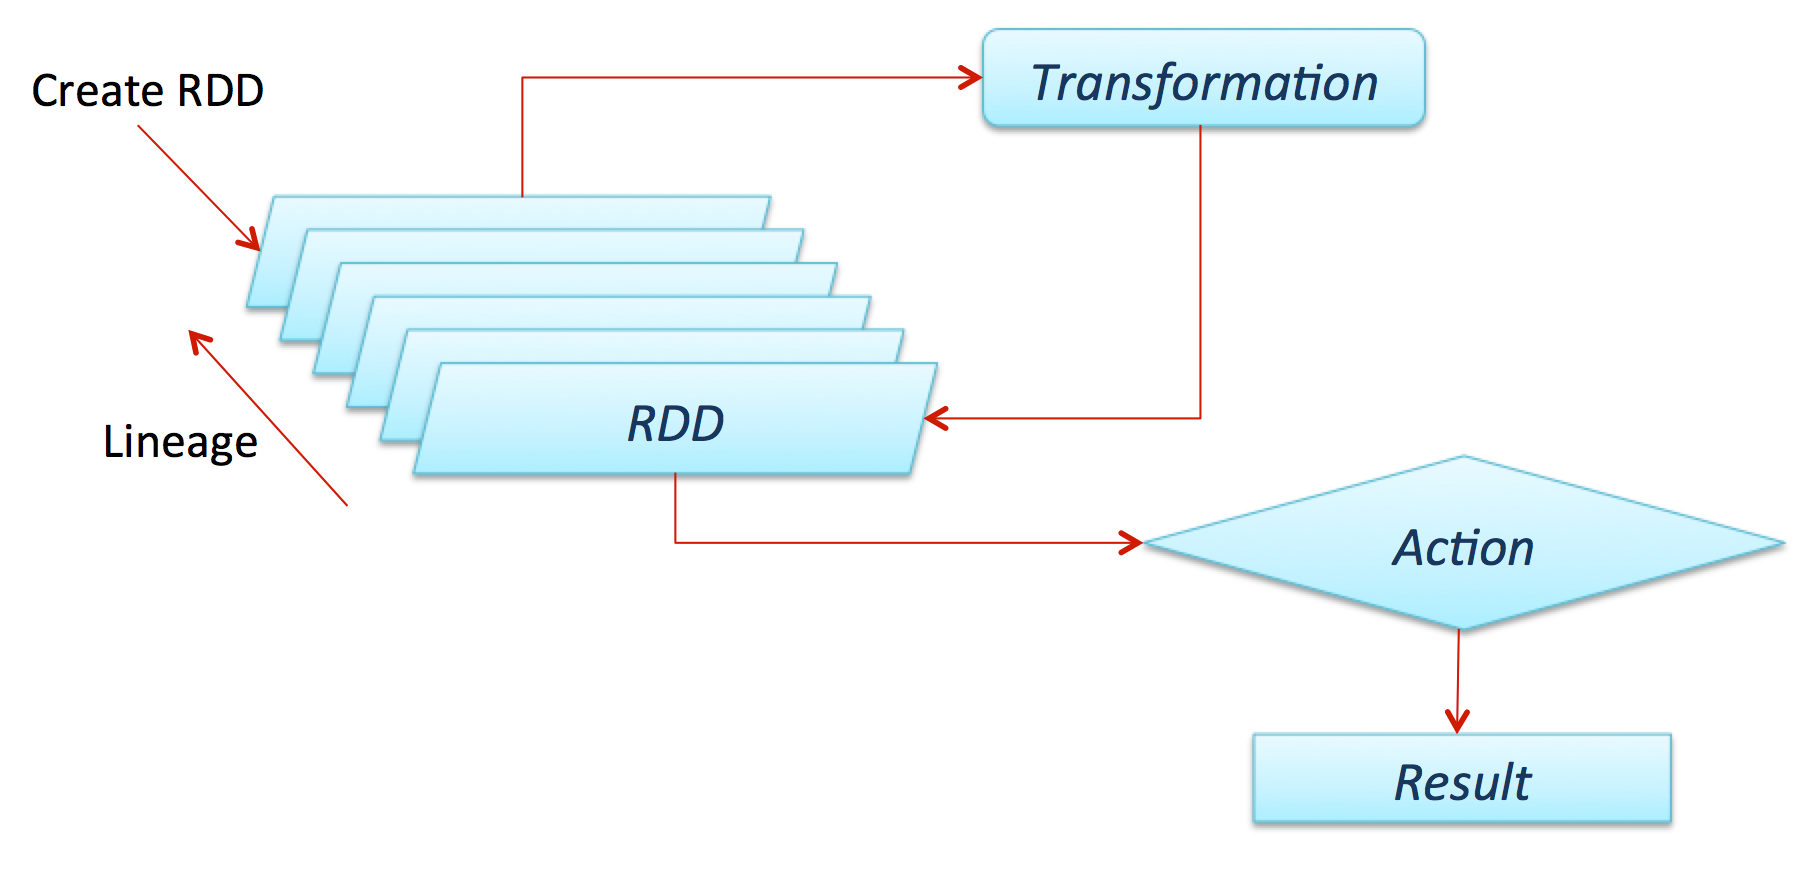
\includegraphics[width=1\textwidth]{img/spark_rdd.png}
    \caption{Operazioni su RDD}
    \label{fig:spark_rdd}
\end{figure}

Nel progetto di Tesi è stato però utilizzato un altro tipo astrazione presente in Spark per memorizzare dati, i \textit{DataFrame}. Sono implementati come degli RDD, pertanto sono anch'essi una collezione di dati distribuiti. La differenza sta nel fatto che sono organizzati in colonne nominate, come avviene nelle tabelle dei database relazionali. Un'altra caratteristica di DataFrame è che le operazioni sono ottimizzabili da Spark mentre le operazioni su RDD sono imperative e passano attraverso le trasformazioni e le azioni in ordine. Questo perfezionamento viene eseguito da un ottimizzatore di query, \textit{Catalyst Optimizer}, che supporta sia l'ottimizzazione basata sulle regole che quella basata sui costi. Nell'ottimizzazione basata su regole, usa un insieme di regole per determinare come eseguire la query. L'ottimizzazione basata sul costo trova il modo più adatto per eseguire l'istruzione. Nell'ottimizzazione basata sui costi, vengono generati più piani utilizzando le regole e poi viene calcolato il loro costo.
\begin{figure}[hbt!]
    \centering
    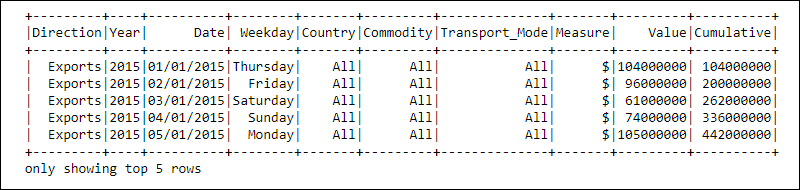
\includegraphics[width=1\textwidth]{img/dataframe_example.png}
    \caption{Esempio di struttura di un DataFrame}
    \label{fig:dataframe_example}
\end{figure}

Durante la fare di sperimentazione, sono stati utilizzati DataFrame per memorizzare i record presenti nei dataset ed effetturare operazioni su di essi. I DataFrame sono stati popolati utilizzando metodi implementati all'interno della struttura dati che permettono di estrarre informazioni da file di diversi formati. Nello specifico sono stati utilizzati per leggere dati da file in formato CSV e CoNLL '03.